\chapter{Zusammenfassung}

Zusammenfassend lässt sich sagen, dass die Umsetzung des Spiels zwar komplizierter war als gedacht, alles in allem aber gut machbar war.

Das Endergebnis ist zwar spielbar, durch die Performanz des Simulators allerdings sehr langsam. Die hier dargestellten Quellcode-Ausschnitte dienen nur zur Illustration der wichtigsten Bestandteile. Der vollständige Quellcode ist in unserem Github-Repository unter https://github.com/flitzpiepe96/Systemnahe-Programmierung einsehbar.

Zum Schluss folgen noch ein paar Bilder aus dem simulierten Programmablauf.

\begin{figure}[htbp]
	\centering
	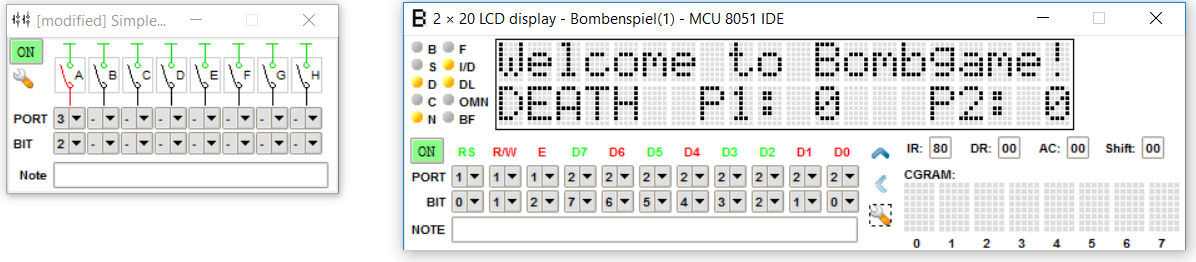
\includegraphics[scale=0.63]{img/Welcome}
	\caption{Willkommensnachricht}
\end{figure}

\begin{figure}[htbp]
	\centering
	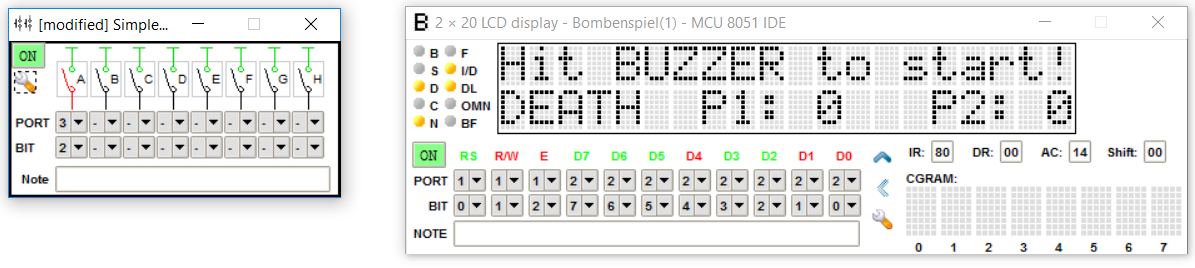
\includegraphics[scale=0.63]{img/StartGame}
	\caption{Startbildschirm}
\end{figure}

\begin{figure}[htbp]
	\centering
	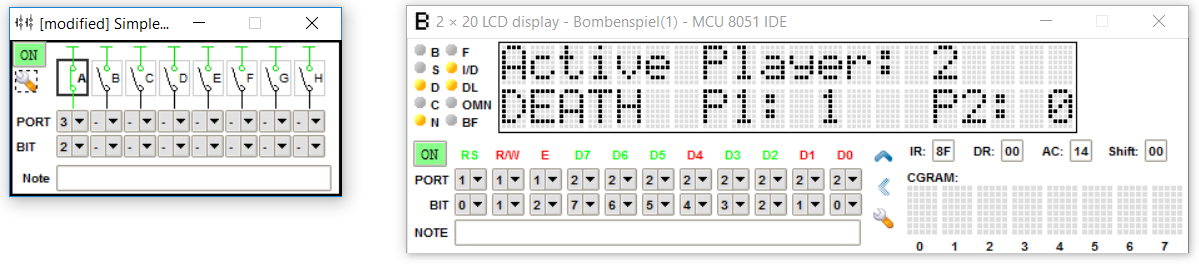
\includegraphics[scale=0.63]{img/Game}
	\caption{Spielablauf}
\end{figure}

\begin{figure}[htbp]
	\centering
	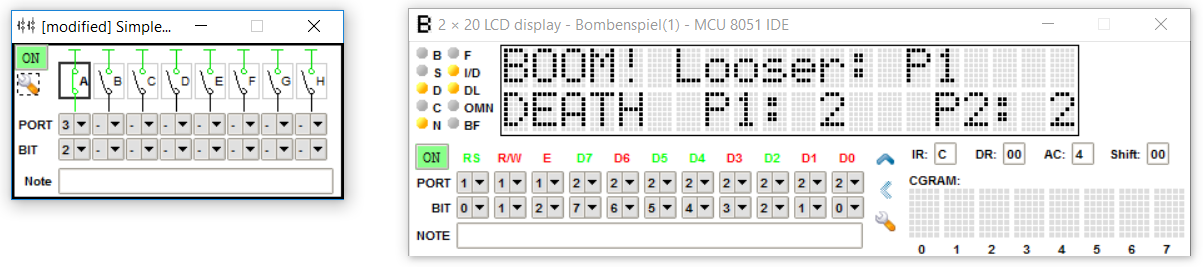
\includegraphics[scale=0.63]{img/Looser}
	\caption{Ende}
\end{figure}